%%
%% This is file `sample-sigchi.tex',
%% generated with the docstrip utility.
%%
%% The original source files were:
%%
%% samples.dtx  (with options: `sigchi')
%% 
%% IMPORTANT NOTICE:
%% 
%% For the copyright see the source file.
%% 
%% Any modified versions of this file must be renamed
%% with new filenames distinct from sample-sigchi.tex.
%% 
%% For distribution of the original source see the terms
%% for copying and modification in the file samples.dtx.
%% 
%% This generated file may be distributed as long as the
%% original source files, as listed above, are part of the
%% same distribution. (The sources need not necessarily be
%% in the same archive or directory.)
%%
%% The first command in your LaTeX source must be the \documentclass command.
\documentclass[sigchi]{acmart}

%%
%% \BibTeX command to typeset BibTeX logo in the docs
\AtBeginDocument{%
  \providecommand\BibTeX{{%
    \normalfont B\kern-0.5em{\scshape i\kern-0.25em b}\kern-0.8em\TeX}}}


%%
%% Submission ID.
%% Use this when submitting an article to a sponsored event. You'll
%% receive a unique submission ID from the organizers
%% of the event, and this ID should be used as the parameter to this command.
%%\acmSubmissionID{123-A56-BU3}

%%
%% The majority of ACM publications use numbered citations and
%% references.  The command \citestyle{authoryear} switches to the
%% "author year" style.
%%
%% If you are preparing content for an event
%% sponsored by ACM SIGGRAPH, you must use the "author year" style of
%% citations and references.
%% Uncommenting
%% the next command will enable that style.
%%\citestyle{acmauthoryear}

%%
%% end of the preamble, start of the body of the document source.
\begin{document}

%%
%% The "title" command has an optional parameter,
%% allowing the author to define a "short title" to be used in page headers.
\title{EEG-Based Brain Disorders Diagnosis through Deep Neural Networks}

%%
%% The "author" command and its associated commands are used to define
%% the authors and their affiliations.
%% Of note is the shared affiliation of the first two authors, and the
%% "authornote" and "authornotemark" commands
%% used to denote shared contribution to the research.
\author{Gabriel A. Maggiotti}
\email{gmaggiotti@gmail.com}
\affiliation{%
  \institution{Jampp.com}
}



%%
%% By default, the full list of authors will be used in the page
%% headers. Often, this list is too long, and will overlap
%% other information printed in the page headers. This command allows
%% the author to define a more concise list
%% of authors' names for this purpose.
\renewcommand{\shortauthors}{Gabriel A. Maggiotti}

%%
%% The abstract is a short summary of the work to be presented in the
%% article.
\begin{abstract}
In most cases, the diagnosis of brain disorders such as epilepsy or a brain tumor is slow and requires endless visits to doctors and electroencephalogram (EEG) technicians. This project aims to automate brain disorder diagnosis by using Artificial Intelligence and deep learning. There are many brain disorders  can be detected by reading an Electroencephalography. Using an EEG device and collecting the electrical signals directly from the brain with a noninvasive procedure gives significant information about its health. Classifying and detecting anomalies on these signals is what doctors currently do when reading an Electroencephalography. With the right amount of data and the use of machine learning models, it could be possible to learn and classify these signals into groups like (i.e: anxiety, epilepsy spikes, abnormal tumor activity, etc). Subsequently, a trained Neural Network would interpret those signals and identify evidence of a disorder to automate the detection and classification of those disorders found. Results are promising, with classification accuracy of 99.69\% for epilepsy and 85.04\% for brain tumor.
\end{abstract}

%%
%% The code below is generated by the tool at http://dl.acm.org/ccs.cfm.
%% Please copy and paste the code instead of the example below.
%%


\ccsdesc[500]{Information Systems~• Life and medical sciences}


%%
%% Keywords. The author(s) should pick words that accurately describe
%% the work being presented. Separate the keywords with commas.
\keywords{datasets, Brain Disorders, EEG, Deep Neural Networks}


%%
%% This command processes the author and affiliation and title
%% information and builds the first part of the formatted document.
\maketitle

\section{Introduction}
This paper explores the use of a supervised machine learning approach to automate the detection of specific disorders on the brain by reading the EEG signals. Primarily, it focuses on Epilepsy and abnormal tumor activities.  Further research could extrapolate this approach to other brain conditions.

Epilepsy is a chronic disorder caused by an imbalance in the electrical activity of neurons in one or several areas of the brain. In most epilepsies, an anomaly in electrical activity can be observed through EEG by registering spikes in the affected areas.  These spikes have a unique pattern that can be seen with the naked eye on an electroencephalogram (spikes or peaks are registered with some frequency associated in the amplitudes of the electrical signals recorded).  Also brain tumors presents a unique pattern in the affected area that can be observed by an EEG.

These marks are indicators of the presence of the disorder. Patients carry this pattern of spikes almost all the time. Seizures or epileptic seizures are events of short duration, being the spikes the catalysts thereof.


\begin{figure}[h]
  \centering
  \includegraphics[width=\linewidth]{media/eeg-spike.eps}
  \caption{Representative abnormal EEG waveforms.}
  \Description{Representative abnormal EEG waveforms.}
\end{figure}

This anomalous brain activity generates an observable mark or pattern. That footprint can be learned through a deep neural network. The following section will elaborate the whole process of data extraction and processing, as well as, the proposed five layers of fully connected Neural Network architecture for feature extraction. Furthermore, the process of training the network with a training-set followed by a validation of the results using a testing/validation set. 


\section{Related work on the subject}
 In the past, similar studies have been conducted using EEG datasets to analyze and make predictions on epilectic seizures and brain tumor related activity. The most common classifiers used were support vector machine (SVM), K Near Neighborhoods (KNN) and Wavelet for datasets like CHB-MIT and UCI database. 

In the recent years more work has been done using neural networks and deep learning models.  Most of these new works present a much better results regardless dataset been used.




\section{Methodology: Dataset Processing}

Dataset used was taken from The University of California Irvine (UCI) [1][2].  UCI contains an Epileptic Seizure Data Set supported by 11500 measurements from a total of 500 individuals with each has 4097 data points for 23.5 seconds and sampling rate of the data was 173.61 Hz. Then divided and shuffled every 4097 data points into 23 chunks, each chunk contains 178 data points for 1 second, and each data point is the value of the EEG recording at a different point in time. So now we have 23 x 500 = 11500 pieces of information(rows), each information contains 178 data points for 1 second(columns), the last column represents the labels.  The dataset contains five different classes of 2300 samples each. Labels 1,2 and 5 were used respectively: class (1 for seizure activity; class (2 for abnormal tumor activity and class (5 for patients without seizures.  

Finally, two dataset were constructed.  For epileptic seizures, samples of classes 1 and 5 were used (4600 samples).  And for brain tumor activity classes 2 and 5 were used with the same number of samples.  
   
\paragraph{}

To avoid saturation on the activation function and to make the gradient descent converge faster, the features were normalized to a range of values between -1 and 1 so that all features have a similar scale Eq.(1). The method used was standardization, which makes every feature have a zero mean Eq.(2) value and unit variance Eq.(3). It is calculated for each feature as follows:


\begin{equation} 
x'=\frac{x-\hat{x}}{\sigma}
\end{equation}

\begin{equation}
\mu (x_{i})= 0   
\end{equation}

\begin{equation} 
\sigma (x_{i}) = \sigma(x_{j})
\end{equation}


\begin{figure}[h]
\centering
\includegraphics[width=8.81cm,height=5.00cm]{media/image7.eps}
\caption{Feature scaling is a method used to standardize the 
range of independent variables or features of data. In data processing, 
it is also known as data normalization and is generally performed during 
the data preprocessing step.}
\end{figure}


Lastly, the dataset was further split into training and validation sets. It is very important that dataset is shuffled well to avoid any element of bias before training the ML model.







\section{Method / The Solution}

Deep learning algorithms are composed of multiple processing layers that learn data representations with multiple levels of abstraction[13]. Using a deep neural networks (DNN) implemented in Python (TensorFlow library), to classify the subjects based on each label.  Design a fully connected Neural Network to capture the nonlinearity of the signals.
 
\paragraph{}
The proposed architecture consists of five layers of fully connected neural networks (Fig. 3), an Adam optimizer[6] was used because it is an efficient extension of stochastic gradient descent optimizers. The Adam optimizer achieves good results faster than other approaches and is used for objective function minimization by iteration. It computes individual adaptive learning rates from estimates of the first and second moments of the gradients. 

\paragraph{}
Parameter initialization included assigning random values between 0 and 1 to the weights Eq.(4) and zero values to the biases. Also, Xavier initialization [3] was applied to the weights following Eq.(5) to make the variance to remain the same as we pass through each layer and preserve the back propagated signal as well.  This helps to reach the minimum of the cost function faster and more efficiently: 

\begin{equation} 
\theta\Rightarrow\theta=\{W_{0},W_{1},W_{2}...,W_{L}\}
\end{equation}

\begin{equation} 
Xavier = \sqrt{\frac{2}{features}}
\end{equation}

The weights were still random, but positive and negative values close to 0 were assigned to produce outputs that followed a similar distribution across all neurons. 


The nonlinear sigmoid function Eq.(7) was applied as the activation function of hidden layers. The objective function used measures the error between the neural networks output and the actual target, as shown in Eq.(8): 

\begin{figure}[h]
\centering
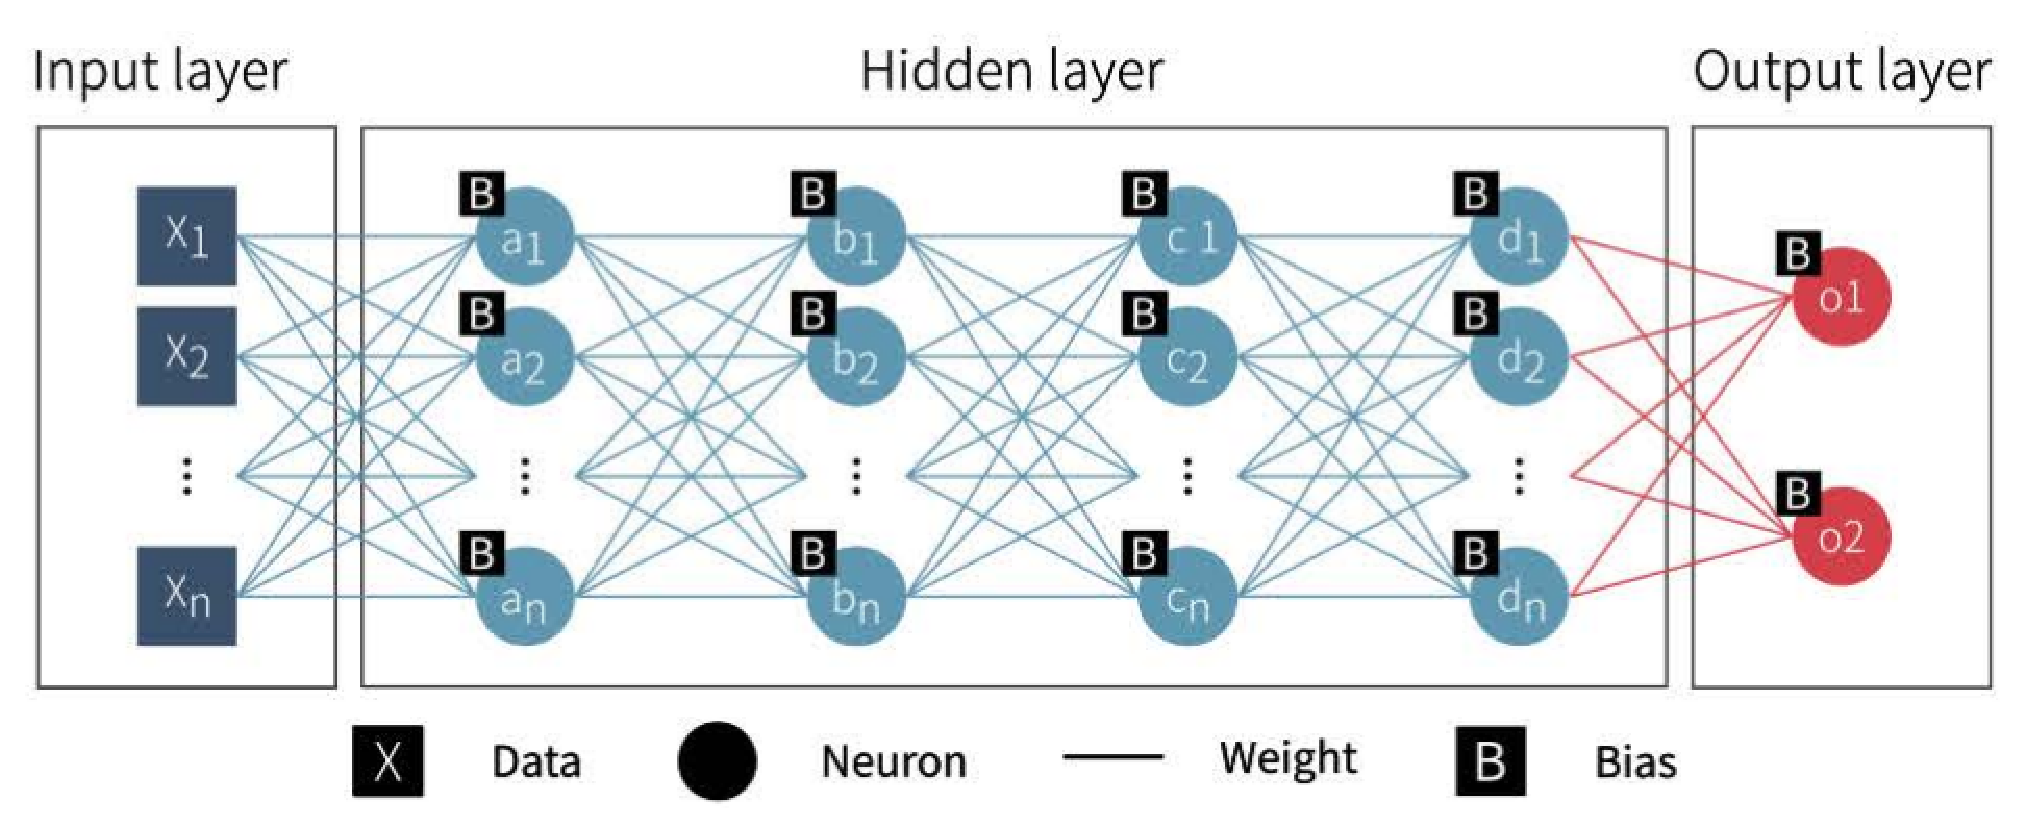
\includegraphics[width=8.51cm,height=3.77cm]{media/deep-nn1.eps}
\caption{Architecture for a four five fully connected 
Neural Network}
\end{figure}


\paragraph{}Iterate for N epochs,  for each training example Xi, Yi 
\begin{equation} 
g(x)^{i+1}=\sum_j^n(x_{j}*w_{j})\Rightarrow X^{i}*W^{i}
\end{equation}

Hidden activation layers are components that introduce non-linearity to 
the system. That Allows to capture and perform very sophisticated type 
of classification functions.
\begin{equation} 
L^{i+1}=sigmoid(g(x)^{i+1})
\end{equation}

\paragraph{}Calculate the error comparing the output of the NN with the actual target 
\begin{equation} 
Error = \frac{1}{2}\sum_i^n( y -\widehat{y})^2
\end{equation}

\begin{equation} 
\widehat{y}=Sigmoid(x_{i}\times w_{i})
\end{equation}

\paragraph{} Use the chain rule to efficiently compute gradients, top to bottom

\begin{equation} 
\frac{\partial E}{\partial w}=\frac{\partial }{\partial w} \frac{1}{2}\sum_i^n( y -\widehat{y})^2
\end{equation}

\begin{equation} 
\frac{\partial E}{\partial w} = \sum_i^n ( y -\widehat{y})  (-\frac{\partial E}{\partial w}\widehat{•}t{y})
\end{equation}

\begin{equation} 
\Rightarrow(\frac{\partial E}{\partial w}\widehat{y})= \widehat{y}(1-\widehat{y})
\end{equation}


\paragraph{}Back propagation of errors using the chain rule
\begin{equation} 
\nabla=\frac{\partial E}{\partial w}
\end{equation}

\begin{equation} 
\nabla_{n-1}=\nabla{n}*W^{T}_{n-1}
\end{equation}


As a regularization procedure for avoiding overfitting, a dropout[7] approach was employed in the fourth hidden layer with a keep probability of 0.5. The optimization procedure was iterated until the minimum error on the training set and the maximum accuracy on the validation set (the number of observations that were correctly classified) were reached (Fig. 4). 
\paragraph{}

\begin{figure}[h]
\centering
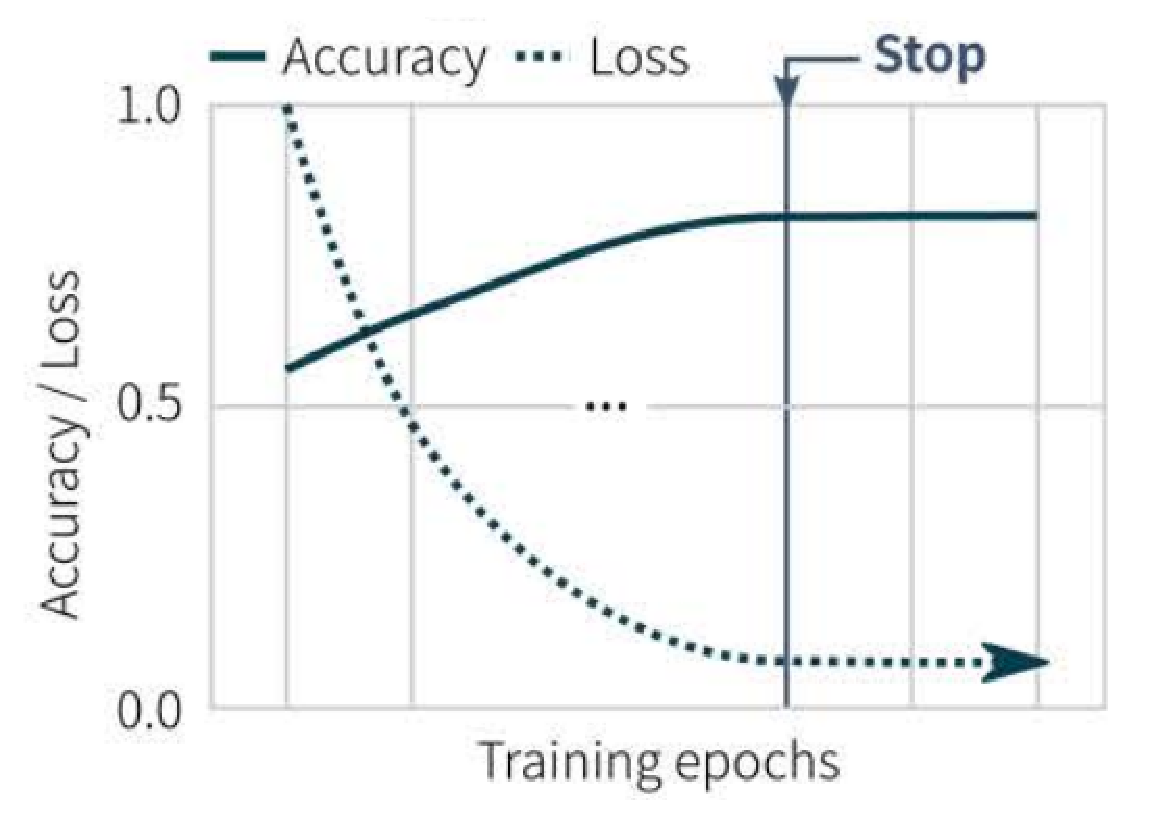
\includegraphics[width=6.08cm,height=5.11cm]{media/training-pro.eps}
\caption{ Training process}
\end{figure}

 A reference to the project and code can be found at [4]. 





\section{Results}

The main model used in the experiments was a five-layer fully-connected neural network with a learning rate of 0.0001, Xavier parameter of 0.8, dropout with a keep probability of 50\%, L2 regularization with a beta of 0.0001, sigmoid activation and exponential decay. 

The model was trained with two datasets, one with patients who had a brain tumor, for whom brain activity was collected in the affected area. The second group was made up of  patients with epileptic seizures.

On the UCI dataset,a three-class classification task was performed. The first group, group A, was comprised of  2300 samples of healthy recordings. The second, group B, was a set of 2300 samples of brain tumor activity recording, The same approach was implemented for epilepsy,  where a set of recordings with epileptic seizures, group  C. Then two datasets were created, A + B for brain tumor classification and A + C for epileptic seizure classification. Both datasets were shuffled and the data was normalized. For each dataset 80\% was taken for training and the remaining 20\% for validation. 


\begin{table}[h!]
\begin{tabular}{ |p{2cm}||p{1.5cm}|p{1.5cm}|p{1.3cm}|p{0.8cm}|  }
 \hline
 \multicolumn{5}{|c|}{Country List} \\
 \hline
 Model     & Dataset &Accuracy \%&Error \%& \# Iterations\\
 \hline
 3 Layer NN & Epilepsy &97.06 +/- 0.14& 1.2 +/- 0.9 &300\\
 5 Layer NN & Epilepsy  & 99.69 +/- 0.05   &0.3 +/- 0.6 &300\\
 5 Layer NN & Brain Tumor & 85.04 +/- 0.08 &  2.99 +/- 0.16 &2760\\
 \hline
\end{tabular}
\caption{ Error and accuracy results for both Epilepsy and Brain Tumor Datasets. +/- is the standard deviation on each set}
\end{table}



\begin{figure}[h]
\centering
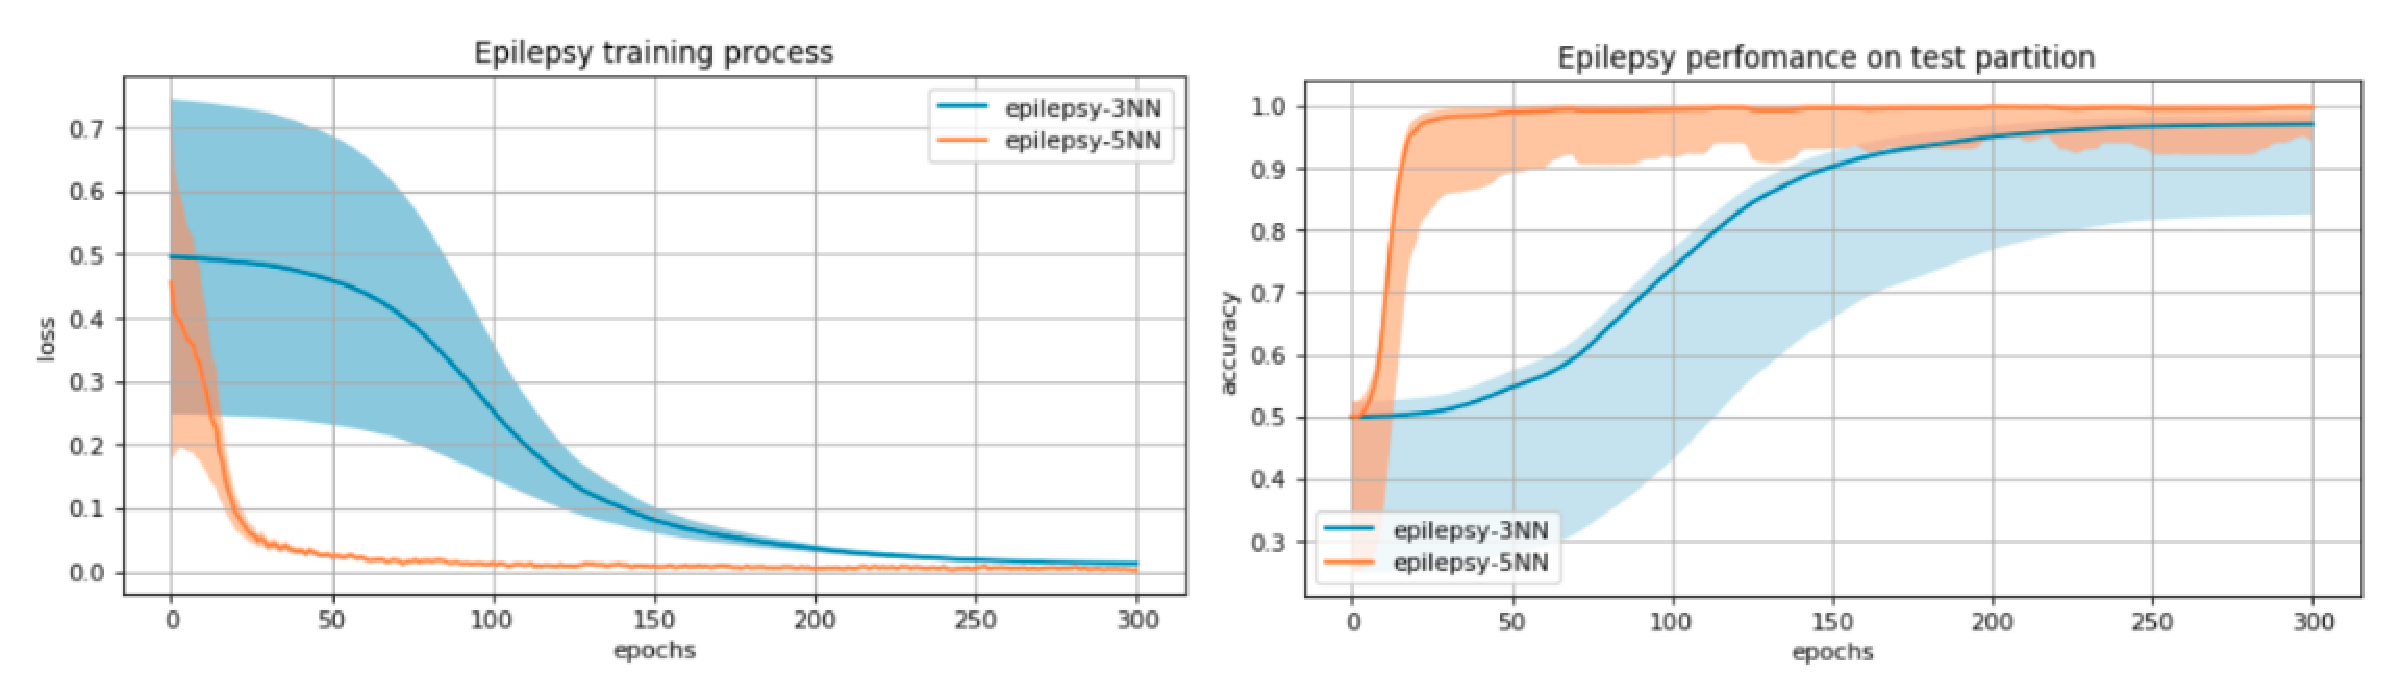
\includegraphics[width=8.5cm,height=3.11cm]{media/results.eps}
\caption{ Error and Accuracy during the training process for the epilepsy dataset.}
\end{figure}


\begin{figure}[h]
\centering
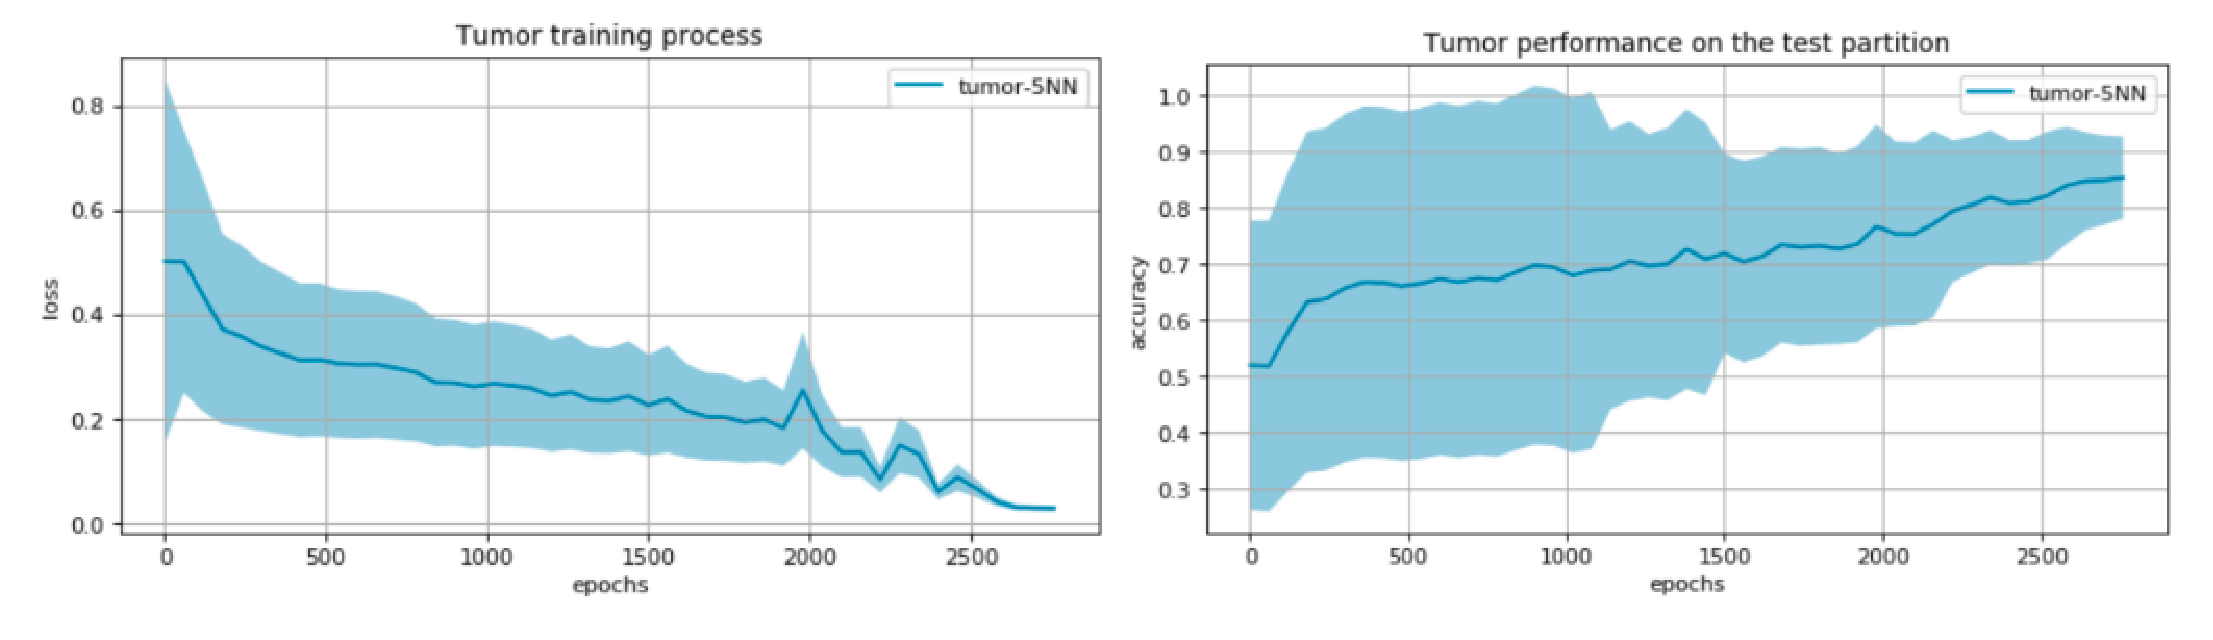
\includegraphics[width=8.5cm,height=3.11cm]{media/results2.eps}
\caption{ Error and Accuracy during the training process for the abnormal tumor activity dataset}
\end{figure}




\section{Conclusion and Future Directions}

A successful automated detection and prediction of disorders introduces new innovative opportunities for diagnosis and preventive health care. This paper proposes a fast and lightway learning procedure for building a predictive model that satisfies the assignment. The use of deep neural networks in the subject turned out to be an excellent solution that presents high accuracy.  

The results are prominent and suggest that the model with existing clinical systems and practices may enable clinicians to make accurate epilepsy diagnosis and start  treatments earlier.

Moreover, it opens a door to extend the work on other areas like diagnosis of dementia, brain damage, brain diseases, psychiatric disorders, stroke, seizure forecasting from the study of interictal, preictal and ictal states and other focal brain disorders. 

Another area of interest would be Electrocardiogram signals. Further works can also be done on predicting heart attacks from ECG signals (people carrying holter monitors). 



% Non-BibTeX users please use
\begin{thebibliography}{}
%
% and use \bibitem to create references. Consult the Instructions
% for authors for reference list style.
%
\bibitem{RefJ}



$[$1$]$ - https://archive.ics.uci.edu/ml/datasets/Epileptic+Seizure +Recognition

$[$2$]$ - Andrzejak RG, Lehnertz K, Rieke C, Mormann F, David P, Elger 
CE (2001) Indications of nonlinear deterministic and finite dimensional 
structures in time series of brain electrical activity: Dependence on 
recording region and brain state, Phys. Rev. E, 64, 061907

$[$3$]$ LeCun, Y., Bengio, Y. and Hinton, G. Deep learning. Nature 521, 436, doi:doi:10.1038/nature14539 (2015).

$[$4$]$ "source code" - https://github.com/gmaggiotti/brain-disorders-prediction

$[$5$]$ Glorot, Xavier and Bengio, Yoshua. (2010) Understanding the difficulty of training deep feedforward neural networks. In Proceedings of the International Conference on Artificial Intelligence and Statistics (AISTATS10). Society for Artificial Intelligence and Statistics.

$[$6$]$ Diederik P. Kingma, Jimmy Lei Ba. (2017) ADAM: A METHOD FOR STOCHASTIC OPTIMIZATION - https://arxiv.org/pdf/1412.6980.pdf

$[$7$]$ Nitish Srivastava, Geoffrey Hinton, Alex Krizhevsky, Ilya Sutskever, Ruslan Salakhutdinov(2014) Dropout: A Simple Way to Prevent Neural Networks from Overfitting


$[$8$]$ Krisztian Buza, Júlia Koller - Classification of Electroencephalograph Data,
A Hubness-aware Approach - https://www.uni-obuda.hu/journal/Buza\_Koller\_66.pdf

$[$9$]$ Pierre Thodorof, Joelle Pineau, Andrew Lim - Learning Robust Features using Deep Learning for Automatic Seizure Detection - https://arxiv.org/pdf/1608.00220.pdf

$[$10$]$ Ihsan Ullah, Muhammad Hussain, Emad-ul-Haq Qaziand Hatim Aboalsamh - An Automated System for Epilepsy Detection using EEG Brain Signals based on Deep Learning Approach - https://arxiv.org/pdf/1801.05412.pdf




\end{thebibliography}


\end{document}
\endinput
%%
%% End of file `sample-sigchi.tex'.
